\section{Механические колебания}

\begin{ex} %Сив557
Построить графики зависимости от времени смещения, скорости и ускорения при простом гармоническом колебании. Построить графики зависимости скорости и ускорения от смещения. Найти соотношения между амплитудами смещения, скорости и ускорения.
\begin{ans}
$v_m = \omega A$, $a_m = \omega^2 A$.
\end{ans}
\end{ex}	

\begin{figure}[h]
\centering
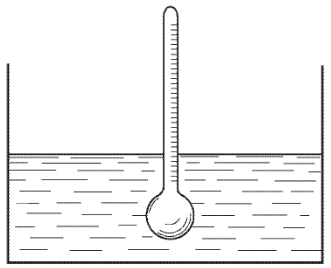
\includegraphics[width=0.35\textwidth]{areometr.png}
\caption{}
\label{areometr}
\end{figure}

\begin{ex} %Сив560
Ареометр с цилиндрической трубкой диаметра $D$ (рис. \ref{areometr}), плавающий в жидкости плотности $\rho$, получает небольшой вертикальный толчок. Найти период колебаний $T$ ареометра, если масса его $m$ известна. Движение жидкости и ее сопротивление движению ареометра не учитывать.
\begin{ans}
$T = 4 \sqrt{\pi m / g \rho D^2}$.
\end{ans}
\end{ex}	

\begin{figure}[h]
\centering
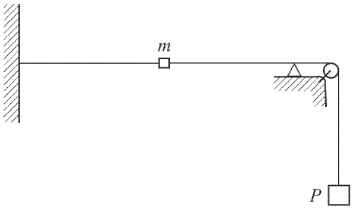
\includegraphics[width=0.5\textwidth]{oscilString.png}
\caption{}
\label{oscilString}
\end{figure}

\begin{ex} %Сив572
Найти период свободных малых колебаний грузика массы $m$, укрепленного на середине тонкой струны длины $L$ (рис. \ref{oscilString}). Массой струны можно пренебречь; натяжение струны постоянно и равно $P$.
\begin{ans}
$T = \pi \sqrt{m L /P}$.
\end{ans}
\end{ex}	

\begin{ex} %Сив580
Горизонтальная мембрана совершает синусоидальные колебания с круговой частотой $\omega$ и и амплитудой $A$. На мембране лежит маленький грузик. При каком условии грузик будет колебаться вместе с мембраной и при каком он начнет подскакивать?
\begin{ans}
При $\omega^2 A > g$ грузик будет подскакивать.
\end{ans}
\end{ex}	

\begin{figure}[h]
\centering
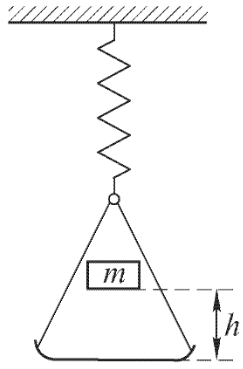
\includegraphics[width=0.25\textwidth]{fallingOnPlate.png}
\caption{}
\label{fallingOnPlate}
\end{figure}

\begin{ex} %Сив582
На чашку весов, подвешенную на пружине, падает с высоты $h$ груз массы $m$ и остается на чашке (рис. \ref{fallingOnPlate}), не подпрыгивая относительно нее. Чашка начинает колебаться. Коэффициент жесткости пружины $k$. Определить амплитуду $A$ колебаний (массой чашки и пружины по сравнению с массой груза можно пренебречь).
\begin{ans}
$A = \frac{mg}{k}\sqrt{ 1 + \frac{2hk}{mg}}$.
\end{ans}
\end{ex}	

\begin{ex} %Сив558
Найти выражения для потенциальной, кинетической и полной энергии материальной точки массы $m$, совершающей гармоническое колебание по закону $A \cos \omega t$.
\begin{ans}
$E_1 = m A^2 \omega^2 (1 - \cos 2 \omega t)/4$, $E_2 = m A^2 \omega^2 (1 + \cos 2 \omega t)/4$, $E = m A^2 \omega^2 /2$.
\end{ans}
\end{ex}	

\begin{ex} %Сив565
Представьте себе шахту, пронизывающую земной шар по одному из его диаметров. Найти закон движения тела, упавшего в эту шахту, учитывая изменения значения ускорения свободного падения внутри Земли. Трение о стенки шахты и сопротивление воздуха не учитывать.
\begin{ans}
Гармоническое колебание с периодом $T = 2 \pi \sqrt{R_0 / g_0}$, где $R_0$ -- радиус земного шара, $g_0$ -- ускорение свободного падения на поверхности Земли.
\end{ans}
\end{ex}	

\begin{figure}[h]
\centering
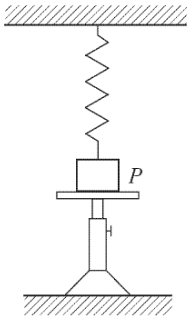
\includegraphics[width=0.25\textwidth]{removePlate.png}
\caption{}
\label{removePlate}
\end{figure}

\begin{ex} %Сив575
К пружине, один конец которой закреплен, подвешен груз $P$ массы $m$, лежащий на подставке так, что пружина не растянута (рис. \ref{removePlate}). Без толчка подставка убирается. Найти движение груза и максимальное натяжение пружины. Коэффициент жесткости пружины $k$.
\begin{ans}
$x = mg/k(1-\cos \sqrt{g/m} t)$.
\end{ans}
\end{ex}	

\begin{ex} %Сив577
На доске лежит груз весом $Р = 10$ Н. Доска совершает гармоническое колебание в вертикальном направлении с периодом $T = 1/2$ с и амплитудой $A = 2$ см. Определить величину силы давления $F$ груза на доску. С какой амплитудой А должна колебаться доска, чтобы груз начал отскакивать от доски?
\begin{ans}
$A \approx 6,2$ см.
\end{ans}
\end{ex}	

\begin{ex} %Сив581
Доска совершает гармоническое колебание в горизонтальном направлении с периодом $T = 5$ с. Лежащее на ней тело начинает скользить, когда амплитуда колебания достигает величины $A = 0,6$ м. Каков коэффициент трения покоя к между грузом и доской?
\begin{ans}
$\mu = 4 \pi^2 A / (gT^2) = 0,1$.
\end{ans}
\end{ex}	

\clearpage